\documentclass[11pt,a4paper]{article}

\usepackage[T1]{fontenc}
\usepackage[utf8]{inputenc}
\usepackage[margin=1in]{geometry}
\usepackage{graphicx}
\usepackage{listings}
\usepackage{xcolor}
\usepackage{parskip}
\usepackage{float}
\usepackage[hidelinks]{hyperref}
\usepackage{longtable}
\usepackage{array}

% ---------------------------------------------------------------
% Listings setup for LLVM IR
% ---------------------------------------------------------------
\definecolor{irkeyword}{RGB}{0,0,180}
\definecolor{irtype}{RGB}{0,120,0}
\definecolor{ircomment}{RGB}{128,128,128}
\definecolor{irback}{RGB}{246,246,246}

\lstdefinelanguage{LLVM}{
  morekeywords={
    alloca,load,store,getelementptr,icmp,fcmp,add,fdiv,br,switch,phi,call,
    ret,sext,sitofp,select,fpext,define,label,inbounds,volatile,align,nsw,
    nuw,slt,eq,oeq,true,false,void,preds,insertelement,shufflevector,
    extractelement
  },
  morekeywords=[2]{i1,i8,i32,i64,ptr,float,double},
  sensitive=true,
  morecomment=[l]{;},
  morestring=[b]",
}

\lstset{
  language=LLVM,
  basicstyle=\ttfamily\small,
  keywordstyle=\color{irkeyword}\bfseries,
  keywordstyle=[2]\color{irtype},
  commentstyle=\color{ircomment}\itshape,
  backgroundcolor=\color{irback},
  frame=single,
  rulecolor=\color{black!25},
  framesep=5pt,
  xleftmargin=6pt,
  xrightmargin=6pt,
  breaklines=true,
  showstringspaces=false,
  columns=fullflexible,
  keepspaces=true,
}

% Inline IR snippet
\newcommand{\ir}[1]{\texttt{#1}}

\begin{document}

\hypersetup{pageanchor=false}
\begin{titlepage}
\centering
\vspace*{1.2cm}

{
\includegraphics[width=4.2cm]{iitd.png}}

\vspace{1.0cm}

{\huge\scshape Indian Institute of Technology Delhi\par}

\vspace{0.4cm}

\vspace{2.2cm}

{\rule{0.85\textwidth}{0.8pt}\par}
\vspace{0.6cm}
{\LARGE\bfseries COL 729 Lab 2: IR and Compiler Passes\par}
\vspace{0.6cm}
{\rule{0.85\textwidth}{0.8pt}\par}

\vspace{2.5cm}

\begin{minipage}{0.45\textwidth}
\centering
{\Large\bfseries Submitted by}\par
\vspace{0.25cm}
{\large Aditya Anand and Varun Subramaniam\par}
{\large 2023CS50284 and 2023CS50497\par}
\end{minipage}%
\begin{minipage}{0.45\textwidth}
\centering
{\Large\bfseries Instructor}\par
\vspace{0.25cm}
{\Large Prof.\ Sorav Bansal\par}
\end{minipage}

\vfill

{\Large 9 September 2026\par}

\vspace{1cm}

\end{titlepage}
\hypersetup{pageanchor=true}
\pagenumbering{arabic}

\section{Opcodes}

All except \texttt{select} are taken from \texttt{opcodes.O0.ll}.
\texttt{select} is from \texttt{opcodes.canonical.ll}.

\subsection*{\texttt{alloca}}

\begin{lstlisting}
13: %1 = alloca i32, align 4
\end{lstlisting}

This line creates a space for a 32-bit integer on the stack (for
\texttt{compiletimeindex}) and \texttt{\%1} is its address. The result type is
\texttt{ptr}.

\subsection*{\texttt{load}}

\begin{lstlisting}
16: %3 = load volatile i32, ptr @runtimeindex, align 4
\end{lstlisting}

This line loads a 32-bit integer \emph{from} \texttt{@runtimeindex} and writes
that value into the SSA name \texttt{\%3}. It does not store into
\texttt{runtimeindex}. The result type is \texttt{i32}.

\subsection*{\texttt{store}}

\begin{lstlisting}
15: store i32 0, ptr %1, align 4
\end{lstlisting}

This stores the value \texttt{0} into the memory that \texttt{\%1} points to
(\texttt{compiletimeindex}). \texttt{\%1} is only the address and it does not
change. \texttt{store} has no result.

\subsection*{\texttt{getelementptr}}

\begin{lstlisting}
18: %5 = getelementptr inbounds [2 x %struct.myStruct], ptr %2, i64 0, i64 %4
\end{lstlisting}

\texttt{\%2} gives the base address of the \texttt{myStruct} array. The first
\texttt{i64 0} moves the pointer by 0 distance forward and changes the pointing
type from a hypothetical array of \texttt{[2 x \%struct.myStruct]} and points to a
\texttt{[2 x \%struct.myStruct]} without moving. The second \texttt{i64 \%4} does pointer
arithmetic with the offset stored in \texttt{\%4} and adds that as offset, so
\texttt{\%5} is the required address. The result type is \texttt{ptr}. This is done in
the line \texttt{arr[runtimeindex].scalar = 1}.
The getelementptr arithmetic is purely done on the addresses. There is no memory access involved. The memory access is done by a separate load/store. Hence, getelementptr does not read the memory.

\subsection*{\texttt{icmp}}

\begin{lstlisting}
46: %5 = icmp slt i32 %4, 3
\end{lstlisting}

This is for integer comparison. It sets the \texttt{\%5} value to true if the
\texttt{\%4} value is less than 3. This is used to check the breaking condition of
the loop in \texttt{f2}. The result type is \texttt{i1}.

\subsection*{\texttt{fcmp}}

\begin{lstlisting}
67: %18 = fcmp oeq double %17, 2.000000e+00
\end{lstlisting}

\texttt{oeq} means that none of the numbers being compared is a NaN and that both the values being compared are equal. This line
checks if \texttt{\%17} is equal to \texttt{2.0f} to check for the break condition in
the loop in \texttt{f2}. The result type is \texttt{i1}.

\subsection*{\texttt{add}}

\begin{lstlisting}
51: %8 = add nsw i32 %7, 1
\end{lstlisting}

\texttt{nsw} means no signed wrap, meaning that no overflow will take place. In
this line 1 is added to \texttt{\%7} to get \texttt{\%8}.

This is the \texttt{loopcarried += 1} step inside the loop in \texttt{f2}.
\texttt{\%7} is the value loaded from \texttt{loopcarried} on line 50. The result
type is \texttt{i32}.

\subsection*{\texttt{fdiv}}

\begin{lstlisting}
55: %11 = fdiv float %10, 2.000000e+00
\end{lstlisting}

The float division value of \texttt{\%10} divided by \texttt{2.0f} is stored in
\texttt{\%11} as done in \texttt{f2}. The result type is \texttt{float}.

\subsection*{\texttt{br}}

\begin{lstlisting}
42: br label %3
\end{lstlisting}

This jumps the eip of the program to the basic block started by label 3.
\texttt{br} has no result.

\subsection*{\texttt{switch}}

\begin{lstlisting}
96: switch i32 %7, label %29 [
\end{lstlisting}

It uses the value of \texttt{\%7} as the switch condition in \texttt{f3}. If it does
not match with anything then the eip changes to \texttt{\%29}. \texttt{switch} has no
result.

\subsection*{\texttt{phi}}

\begin{lstlisting}
120: %16 = phi i32 [ %13, %12 ], [ 7, %14 ]
\end{lstlisting}

It changes this line \texttt{int t = (runtimeindex > 1) ? loopcarried : 7;}.
Clang emits it as 4 basic blocks \texttt{\%9}, \texttt{\%12}, \texttt{\%14}, \texttt{\%15}; the phi
does not create them. The phi sits at the join block \texttt{\%15} and picks \texttt{\%13}
if control came from \texttt{\%12} and 7 if it came from \texttt{\%14}, so that SSA is not
broken. The result type is \texttt{i32}.

\subsection*{\texttt{call}}

\begin{lstlisting}
104: call void @f1()
\end{lstlisting}

Calls the function \texttt{f1}. It is the first case of the switch. \texttt{f1}
returns void so there is no result.

\subsection*{\texttt{ret}}

\begin{lstlisting}
34: ret void
\end{lstlisting}

It returns void at the end of \texttt{f1}. \texttt{ret} has no result.

\subsection*{\texttt{sext}}

\begin{lstlisting}
17: %4 = sext i32 %3 to i64
\end{lstlisting}

It is a \texttt{sext} (signed extension) of the value of \texttt{\%3} from 32 to 64
bits because pointer arithmetic is done in 64 bits. The result type is
\texttt{i64}.

\subsection*{\texttt{sitofp}}

\begin{lstlisting}
54: %10 = sitofp i32 %9 to float
\end{lstlisting}

It is used in this line \texttt{float myf = loopcarried/2.0f;}. \texttt{\%9} is the
\texttt{loopcarried} value, which is converted into a float register \texttt{\%10}
before doing arithmetic. The result type is \texttt{float}.

\subsection*{\texttt{select}}

\begin{lstlisting}
71: %4 = select i1 %2, i32 %3, i32 7
\end{lstlisting}

It changes this line \texttt{int t = (runtimeindex > 1) ? loopcarried : 7;}.
Instead of using 2 basic blocks to first calculate the values and using phi, it
is storing the result of the comparison in \texttt{\%2} and using its result directly
to take from one of the branches. The result type is \texttt{i32}.

\section{Control Flow Graph}

\begin{figure}[H]
  \centering
  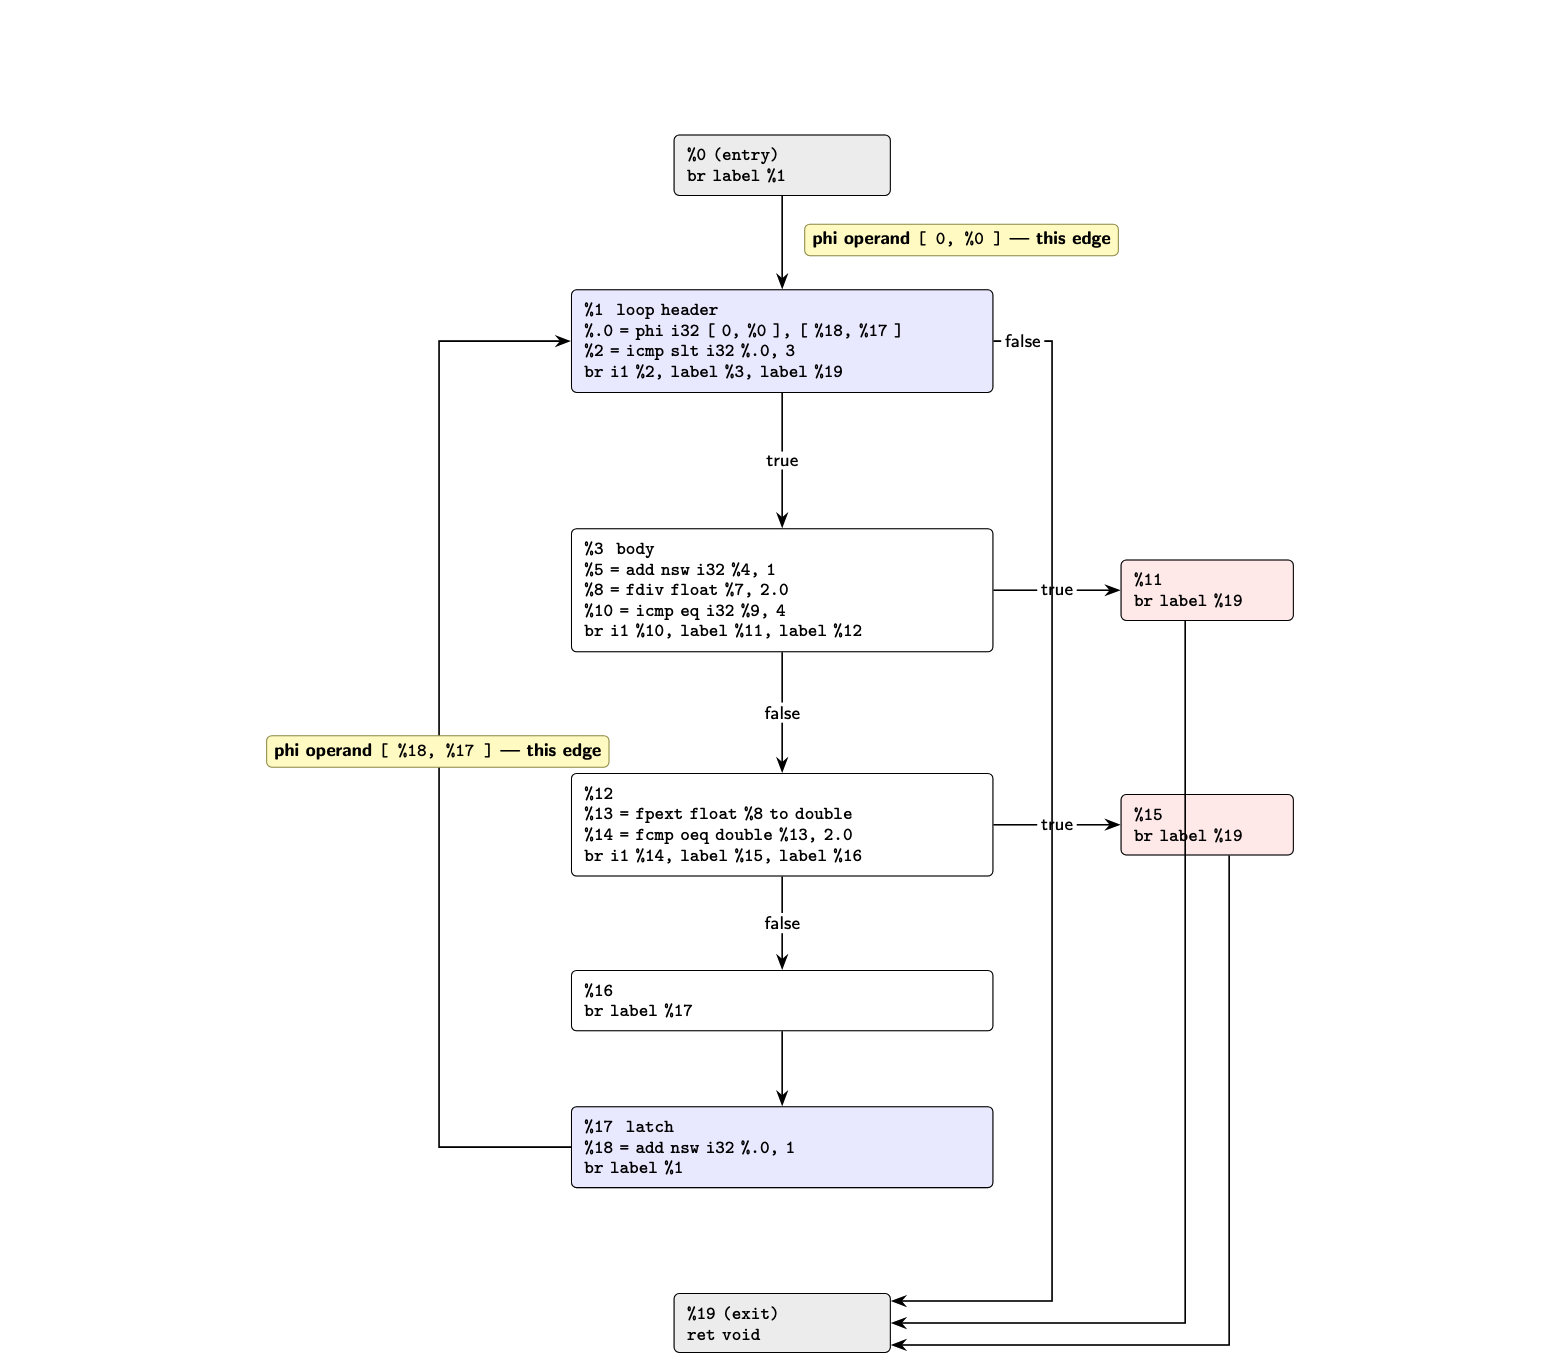
\includegraphics[width=\textwidth]{cfg.png}
  \caption{Control flow graph.}
\end{figure}

\section{\texttt{opcodes.mem2reg.ll}}

\subsection*{Explaining struct access}

\begin{lstlisting}
%5 = getelementptr inbounds [2 x %struct.myStruct], ptr %2, i64 0, i64 %4
%6 = getelementptr inbounds nuw %struct.myStruct, ptr %5, i32 0, i32 0
\end{lstlisting}

The layout of \texttt{myStruct} on this target is: \texttt{scalar} at offset 0,
\texttt{array[2][2]} at bytes 4--19, 4 bytes of padding so the pointer is
aligned, \texttt{ptr} at offset 24, total size 32, alignment 8.

First GEP: \texttt{\%2} is the base of the \texttt{arr} allocation.
\texttt{i64 0} treats that pointer as pointing at one
\texttt{[2 x \%struct.myStruct]} and does not move it.
\texttt{i64 \%4} is the run-time index \texttt{runtimeindex}. That steps by
the \emph{struct} size, so the address is
\texttt{base + 32 * runtimeindex}. Result: pointer to
\texttt{arr[runtimeindex]}.

Second GEP: the first \texttt{i32 0} is ``this struct, no extra stride''.
The second \texttt{i32 0} is field 0, which is \texttt{.scalar}. That field
is at offset \textbf{0}, not $32 \times$ anything. 32 bytes is only the
size of one \texttt{myStruct}, used by the array-element index above.

The getelementptr arithmetic is purely done on the addresses. There is no
memory access involved. The memory access is done by a separate load/store.
Hence, getelementptr does not read the memory.

\section{Part B}

\begin{figure}[H]
  \centering
  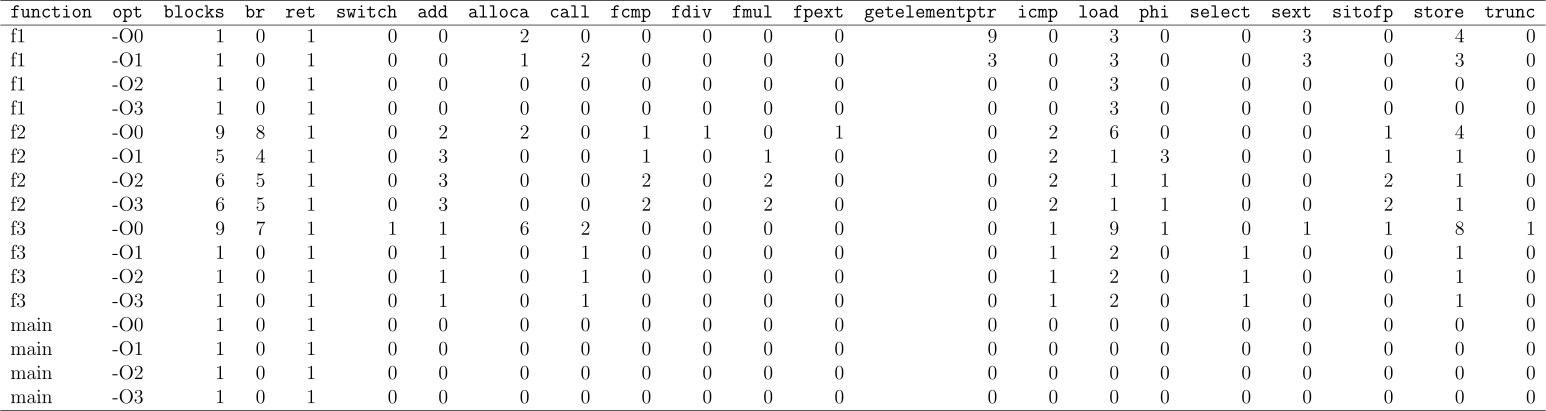
\includegraphics[width=\textwidth]{opcode_table.png}
  \caption{Opcode counts per function and optimisation level.}
\end{figure}

\subsection*{1)}

\textbf{Before:}

\begin{lstlisting}
%1 = alloca i32, align 4
store i32 0, ptr %1, align 4
br label %3

3:
%4 = load i32, ptr %1, align 4
%5 = icmp slt i32 %4, 3
br i1 %5, label %6, label %24

21:
%22 = load i32, ptr %1, align 4
%23 = add nsw i32 %22, 1
store i32 %23, ptr %1, align 4
br label %3, !llvm.loop !5
\end{lstlisting}

\textbf{After} \texttt{opt -S -passes=mem2reg opcodes.O0.ll}:

\begin{lstlisting}
br label %1

1:
%.0 = phi i32 [ 0, %0 ], [ %18, %17 ]
%2 = icmp slt i32 %.0, 3
...

17:
%18 = add nsw i32 %.0, 1
br label %1, !llvm.loop !5
\end{lstlisting}

\textbf{Explanation:} Change made by \texttt{mem2reg}. In \texttt{f2}, the loop
counter becomes a phi node. Earlier the loop counter was in the stack slot. Now
it is promoted to a register.

\subsection*{2)}

\texttt{f3} switches on \texttt{int a = 1}. At \texttt{-O0} the switch and
all four cases are still there (9 blocks, one \texttt{switch}). Cases 0, 2
and 3 are dead.

\textbf{Before} (\texttt{opcodes.O0.ll}):

\begin{lstlisting}
store i32 1, ptr %1, align 4
%6 = load i32, ptr %1, align 4
switch i32 %6, label %31 [
  i32 0, label %7
  i32 1, label %8
  i32 2, label %19
  i32 3, label %25
]
\end{lstlisting}

\textbf{After} \texttt{opt -S -passes='function(mem2reg,sccp,simplifycfg)'}:

\begin{lstlisting}
%1 = load volatile i32, ptr @runtimeindex, align 4
%2 = icmp sgt i32 %1, 1
%3 = load i32, ptr @loopcarried, align 4
%4 = select i1 %2, i32 %3, i32 7
%5 = load i32, ptr @loopcarried, align 4
%6 = add nsw i32 %5, %4
store i32 %6, ptr @loopcarried, align 4
call void @f1()
ret void
\end{lstlisting}

\texttt{sccp} sees that the switch condition is the constant 1.
\texttt{simplifycfg} deletes the unused arms and the \texttt{switch}.
What is left is only case 1: the ternary becomes a \texttt{select}, then
\texttt{call @f1}. That is why the Part B table goes from 9 blocks to 1
and from one \texttt{switch} to zero at \texttt{-O1}. This is not
\texttt{mem2reg}; \texttt{mem2reg} alone still leaves the four cases.

\subsection*{3)}

\textbf{Before:}

\begin{lstlisting}
3:                                                ; preds = %1
%9 = load i32, ptr @loopcarried, align 4
%10 = icmp eq i32 %9, 4
br i1 %10, label %11, label %12

11:                                               ; preds = %3
br label %19

12:                                               ; preds = %3
%13 = fpext float %8 to double
%14 = fcmp oeq double %13, 2.000000e+00
br i1 %14, label %15, label %16

15:                                               ; preds = %12
br label %19

16:                                               ; preds = %12
br label %17
\end{lstlisting}

\textbf{After:}

\begin{lstlisting}
3:                                                ; preds = %1
%9 = load i32, ptr @loopcarried, align 4
%10 = icmp eq i32 %9, 4
%11 = fpext float %8 to double
%12 = fcmp oeq double %11, 2.000000e+00
%or.cond = select i1 %10, i1 true, i1 %12
br i1 %or.cond, label %15, label %13
\end{lstlisting}

The before code is after \texttt{opt -S -passes=mem2reg opcodes.O0.ll}.
The after code is after
\texttt{opt -S -passes='mem2reg,simplifycfg' opcodes.O0.ll}.

It collapses the 2 statements in the code:

\begin{lstlisting}[language={}]
if (loopcarried == 4) break;
else if (myf == 2.0) break;
\end{lstlisting}

into a common \texttt{or.cond} check, simplifying the branch specification.

\section{Part C}

These numbers are from Homebrew LLVM 18.1.8 on arm64 macOS
(\texttt{opt --version}), the same install used for \texttt{clang}.

The pipeline was dumped with
\texttt{opt -passes="default<On>" -print-pipeline-passes}.
Names followed by \texttt{(...)} are adaptors
(\texttt{function}, \texttt{cgscc}, \texttt{loop}, \texttt{loop-mssa},
\texttt{devirt}, \texttt{coro-cond}) and were dropped.
\texttt{require<>}, \texttt{invalidate<>}, \texttt{recompute-globalsaa},
\texttt{verify}, \texttt{annotation-remarks}, \texttt{transform-warning} and
\texttt{cg-profile} were dropped because they are analyses or instrumentation.
\texttt{AArch64LoopIdiomTransformPass} showed up in the dump but it is a C++
class name and cannot be written in \texttt{-passes='...'}, so it was skipped.
Repeats were kept, in order.

\subsection*{Counts}

\begin{tabular}{lrr}
\hline
level & invocations & distinct \\
\hline
\texttt{-O0} & 5 & 5 \\
\texttt{-O1} & 81 & 55 \\
\texttt{-O2} & 97 & 66 \\
\texttt{-O3} & 100 & 69 \\
\hline
\end{tabular}

\subsection*{Ordered lists}

Same order as the dump, one column per level. Type is small so each
name stays on one line. What each name does is in the table below;
the numbers there are how many times it ran.

{\fontsize{5.4pt}{6.6pt}\selectfont
\setlength{\tabcolsep}{5pt}
\renewcommand{\arraystretch}{1.15}
\begin{longtable}{llll}
\hline
\texttt{-O0} & \texttt{-O1} & \texttt{-O2} & \texttt{-O3} \\
\hline
\endfirsthead
\hline
\texttt{-O0} & \texttt{-O1} & \texttt{-O2} & \texttt{-O3} \\
\hline
\endhead
1.~\texttt{always-inline} & 1.~\texttt{annotation2metadata} & 1.~\texttt{annotation2metadata} & 1.~\texttt{annotation2metadata} \\
2.~\texttt{coro-early} & 2.~\texttt{forceattrs} & 2.~\texttt{forceattrs} & 2.~\texttt{forceattrs} \\
3.~\texttt{coro-split} & 3.~\texttt{inferattrs} & 3.~\texttt{inferattrs} & 3.~\texttt{inferattrs} \\
4.~\texttt{coro-cleanup} & 4.~\texttt{coro-early} & 4.~\texttt{coro-early} & 4.~\texttt{coro-early} \\
5.~\texttt{globaldce} & 5.~\texttt{lower-expect} & 5.~\texttt{lower-expect} & 5.~\texttt{lower-expect} \\
 & 6.~\texttt{simplifycfg} & 6.~\texttt{simplifycfg} & 6.~\texttt{simplifycfg} \\
 & 7.~\texttt{sroa} & 7.~\texttt{sroa} & 7.~\texttt{sroa} \\
 & 8.~\texttt{early-cse} & 8.~\texttt{early-cse} & 8.~\texttt{early-cse} \\
 & 9.~\texttt{openmp-opt} & 9.~\texttt{openmp-opt} & 9.~\texttt{callsite-splitting} \\
 & 10.~\texttt{ipsccp} & 10.~\texttt{ipsccp} & 10.~\texttt{openmp-opt} \\
 & 11.~\texttt{called-value-propagation} & 11.~\texttt{called-value-propagation} & 11.~\texttt{ipsccp} \\
 & 12.~\texttt{globalopt} & 12.~\texttt{globalopt} & 12.~\texttt{called-value-propagation} \\
 & 13.~\texttt{mem2reg} & 13.~\texttt{mem2reg} & 13.~\texttt{globalopt} \\
 & 14.~\texttt{instcombine} & 14.~\texttt{instcombine} & 14.~\texttt{mem2reg} \\
 & 15.~\texttt{simplifycfg} & 15.~\texttt{simplifycfg} & 15.~\texttt{instcombine} \\
 & 16.~\texttt{always-inline} & 16.~\texttt{always-inline} & 16.~\texttt{simplifycfg} \\
 & 17.~\texttt{inline} & 17.~\texttt{inline} & 17.~\texttt{always-inline} \\
 & 18.~\texttt{function-attrs} & 18.~\texttt{function-attrs} & 18.~\texttt{inline} \\
 & 19.~\texttt{sroa} & 19.~\texttt{openmp-opt-cgscc} & 19.~\texttt{function-attrs} \\
 & 20.~\texttt{early-cse} & 20.~\texttt{sroa} & 20.~\texttt{argpromotion} \\
 & 21.~\texttt{simplifycfg} & 21.~\texttt{early-cse} & 21.~\texttt{openmp-opt-cgscc} \\
 & 22.~\texttt{instcombine} & 22.~\texttt{speculative-execution} & 22.~\texttt{sroa} \\
 & 23.~\texttt{libcalls-shrinkwrap} & 23.~\texttt{jump-threading} & 23.~\texttt{early-cse} \\
 & 24.~\texttt{simplifycfg} & 24.~\texttt{correlated-propagation} & 24.~\texttt{speculative-execution} \\
 & 25.~\texttt{reassociate} & 25.~\texttt{simplifycfg} & 25.~\texttt{jump-threading} \\
 & 26.~\texttt{loop-instsimplify} & 26.~\texttt{instcombine} & 26.~\texttt{correlated-propagation} \\
 & 27.~\texttt{loop-simplifycfg} & 27.~\texttt{aggressive-instcombine} & 27.~\texttt{simplifycfg} \\
 & 28.~\texttt{licm} & 28.~\texttt{libcalls-shrinkwrap} & 28.~\texttt{instcombine} \\
 & 29.~\texttt{loop-rotate} & 29.~\texttt{tailcallelim} & 29.~\texttt{aggressive-instcombine} \\
 & 30.~\texttt{licm} & 30.~\texttt{simplifycfg} & 30.~\texttt{libcalls-shrinkwrap} \\
 & 31.~\texttt{simple-loop-unswitch} & 31.~\texttt{reassociate} & 31.~\texttt{tailcallelim} \\
 & 32.~\texttt{simplifycfg} & 32.~\texttt{constraint-elimination} & 32.~\texttt{simplifycfg} \\
 & 33.~\texttt{instcombine} & 33.~\texttt{loop-instsimplify} & 33.~\texttt{reassociate} \\
 & 34.~\texttt{loop-idiom} & 34.~\texttt{loop-simplifycfg} & 34.~\texttt{constraint-elimination} \\
 & 35.~\texttt{indvars} & 35.~\texttt{licm} & 35.~\texttt{loop-instsimplify} \\
 & 36.~\texttt{loop-deletion} & 36.~\texttt{loop-rotate} & 36.~\texttt{loop-simplifycfg} \\
 & 37.~\texttt{loop-unroll-full} & 37.~\texttt{licm} & 37.~\texttt{licm} \\
 & 38.~\texttt{sroa} & 38.~\texttt{simple-loop-unswitch} & 38.~\texttt{loop-rotate} \\
 & 39.~\texttt{memcpyopt} & 39.~\texttt{simplifycfg} & 39.~\texttt{licm} \\
 & 40.~\texttt{sccp} & 40.~\texttt{instcombine} & 40.~\texttt{simple-loop-unswitch} \\
 & 41.~\texttt{bdce} & 41.~\texttt{loop-idiom} & 41.~\texttt{simplifycfg} \\
 & 42.~\texttt{instcombine} & 42.~\texttt{indvars} & 42.~\texttt{instcombine} \\
 & 43.~\texttt{coro-elide} & 43.~\texttt{loop-deletion} & 43.~\texttt{loop-idiom} \\
 & 44.~\texttt{adce} & 44.~\texttt{loop-unroll-full} & 44.~\texttt{indvars} \\
 & 45.~\texttt{simplifycfg} & 45.~\texttt{sroa} & 45.~\texttt{loop-deletion} \\
 & 46.~\texttt{instcombine} & 46.~\texttt{vector-combine} & 46.~\texttt{loop-unroll-full} \\
 & 47.~\texttt{function-attrs} & 47.~\texttt{mldst-motion} & 47.~\texttt{sroa} \\
 & 48.~\texttt{coro-split} & 48.~\texttt{gvn} & 48.~\texttt{vector-combine} \\
 & 49.~\texttt{deadargelim} & 49.~\texttt{sccp} & 49.~\texttt{mldst-motion} \\
 & 50.~\texttt{coro-cleanup} & 50.~\texttt{bdce} & 50.~\texttt{gvn} \\
 & 51.~\texttt{globalopt} & 51.~\texttt{instcombine} & 51.~\texttt{sccp} \\
 & 52.~\texttt{globaldce} & 52.~\texttt{jump-threading} & 52.~\texttt{bdce} \\
 & 53.~\texttt{elim-avail-extern} & 53.~\texttt{correlated-propagation} & 53.~\texttt{instcombine} \\
 & 54.~\texttt{rpo-function-attrs} & 54.~\texttt{adce} & 54.~\texttt{jump-threading} \\
 & 55.~\texttt{float2int} & 55.~\texttt{memcpyopt} & 55.~\texttt{correlated-propagation} \\
 & 56.~\texttt{lower-constant-intrinsics} & 56.~\texttt{dse} & 56.~\texttt{adce} \\
 & 57.~\texttt{loop-rotate} & 57.~\texttt{move-auto-init} & 57.~\texttt{memcpyopt} \\
 & 58.~\texttt{loop-deletion} & 58.~\texttt{licm} & 58.~\texttt{dse} \\
 & 59.~\texttt{loop-distribute} & 59.~\texttt{coro-elide} & 59.~\texttt{move-auto-init} \\
 & 60.~\texttt{inject-tli-mappings} & 60.~\texttt{simplifycfg} & 60.~\texttt{licm} \\
 & 61.~\texttt{loop-vectorize} & 61.~\texttt{instcombine} & 61.~\texttt{coro-elide} \\
 & 62.~\texttt{infer-alignment} & 62.~\texttt{function-attrs} & 62.~\texttt{simplifycfg} \\
 & 63.~\texttt{loop-load-elim} & 63.~\texttt{coro-split} & 63.~\texttt{instcombine} \\
 & 64.~\texttt{instcombine} & 64.~\texttt{deadargelim} & 64.~\texttt{function-attrs} \\
 & 65.~\texttt{simplifycfg} & 65.~\texttt{coro-cleanup} & 65.~\texttt{coro-split} \\
 & 66.~\texttt{vector-combine} & 66.~\texttt{globalopt} & 66.~\texttt{deadargelim} \\
 & 67.~\texttt{instcombine} & 67.~\texttt{globaldce} & 67.~\texttt{coro-cleanup} \\
 & 68.~\texttt{loop-unroll} & 68.~\texttt{elim-avail-extern} & 68.~\texttt{globalopt} \\
 & 69.~\texttt{sroa} & 69.~\texttt{rpo-function-attrs} & 69.~\texttt{globaldce} \\
 & 70.~\texttt{infer-alignment} & 70.~\texttt{float2int} & 70.~\texttt{elim-avail-extern} \\
 & 71.~\texttt{instcombine} & 71.~\texttt{lower-constant-intrinsics} & 71.~\texttt{rpo-function-attrs} \\
 & 72.~\texttt{licm} & 72.~\texttt{loop-rotate} & 72.~\texttt{float2int} \\
 & 73.~\texttt{alignment-from-assumptions} & 73.~\texttt{loop-deletion} & 73.~\texttt{lower-constant-intrinsics} \\
 & 74.~\texttt{loop-sink} & 74.~\texttt{loop-distribute} & 74.~\texttt{chr} \\
 & 75.~\texttt{instsimplify} & 75.~\texttt{inject-tli-mappings} & 75.~\texttt{loop-rotate} \\
 & 76.~\texttt{div-rem-pairs} & 76.~\texttt{loop-vectorize} & 76.~\texttt{loop-deletion} \\
 & 77.~\texttt{tailcallelim} & 77.~\texttt{infer-alignment} & 77.~\texttt{loop-distribute} \\
 & 78.~\texttt{simplifycfg} & 78.~\texttt{loop-load-elim} & 78.~\texttt{inject-tli-mappings} \\
 & 79.~\texttt{globaldce} & 79.~\texttt{instcombine} & 79.~\texttt{loop-vectorize} \\
 & 80.~\texttt{constmerge} & 80.~\texttt{simplifycfg} & 80.~\texttt{infer-alignment} \\
 & 81.~\texttt{rel-lookup-table-converter} & 81.~\texttt{slp-vectorizer} & 81.~\texttt{loop-load-elim} \\
 &  & 82.~\texttt{vector-combine} & 82.~\texttt{instcombine} \\
 &  & 83.~\texttt{instcombine} & 83.~\texttt{simplifycfg} \\
 &  & 84.~\texttt{loop-unroll} & 84.~\texttt{slp-vectorizer} \\
 &  & 85.~\texttt{sroa} & 85.~\texttt{vector-combine} \\
 &  & 86.~\texttt{infer-alignment} & 86.~\texttt{instcombine} \\
 &  & 87.~\texttt{instcombine} & 87.~\texttt{loop-unroll} \\
 &  & 88.~\texttt{licm} & 88.~\texttt{sroa} \\
 &  & 89.~\texttt{alignment-from-assumptions} & 89.~\texttt{infer-alignment} \\
 &  & 90.~\texttt{loop-sink} & 90.~\texttt{instcombine} \\
 &  & 91.~\texttt{instsimplify} & 91.~\texttt{licm} \\
 &  & 92.~\texttt{div-rem-pairs} & 92.~\texttt{alignment-from-assumptions} \\
 &  & 93.~\texttt{tailcallelim} & 93.~\texttt{loop-sink} \\
 &  & 94.~\texttt{simplifycfg} & 94.~\texttt{instsimplify} \\
 &  & 95.~\texttt{globaldce} & 95.~\texttt{div-rem-pairs} \\
 &  & 96.~\texttt{constmerge} & 96.~\texttt{tailcallelim} \\
 &  & 97.~\texttt{rel-lookup-table-converter} & 97.~\texttt{simplifycfg} \\
 &  &  & 98.~\texttt{globaldce} \\
 &  &  & 99.~\texttt{constmerge} \\
 &  &  & 100.~\texttt{rel-lookup-table-converter} \\
\hline
\end{longtable}
}

\subsection*{Pass descriptions}

{\small
\begin{longtable}{lp{5.6cm}rrrr}
\hline
pass & description & \texttt{-O0} & \texttt{-O1} & \texttt{-O2} & \texttt{-O3} \\
\hline
\endfirsthead
\hline
pass & description & \texttt{-O0} & \texttt{-O1} & \texttt{-O2} & \texttt{-O3} \\
\hline
\endhead
\texttt{adce} & deletes dead code even if it is only dead on some paths & 0 & 1 & 1 & 1 \\
\texttt{aggressive-instcombine} & extra instcombine work the cheap pass will not touch & 0 & 0 & 1 & 1 \\
\texttt{alignment-from-assumptions} & if an assume says the pointer is aligned, mark the load/store that way & 0 & 1 & 1 & 1 \\
\texttt{always-inline} & inlines \texttt{always\_inline} functions; this is why it still runs at \texttt{-O0} & 1 & 1 & 1 & 1 \\
\texttt{annotation2metadata} & turns the old annotation globals into metadata & 0 & 1 & 1 & 1 \\
\texttt{argpromotion} & if you only pass a pointer to read one field, just pass the field & 0 & 0 & 0 & 1 \\
\texttt{bdce} & DCE that also drops unused \emph{bits}, not just unused values & 0 & 1 & 1 & 1 \\
\texttt{called-value-propagation} & if a call always hits the same function, put that name in & 0 & 1 & 1 & 1 \\
\texttt{callsite-splitting} & clones a call so each incoming edge can see a constant & 0 & 0 & 0 & 1 \\
\texttt{chr} & flattens a pile of hot ifs so the common path is shorter & 0 & 0 & 0 & 1 \\
\texttt{constmerge} & one copy of the same constant string / array & 0 & 1 & 1 & 1 \\
\texttt{constraint-elimination} & if an earlier icmp already proved this one, fold it & 0 & 0 & 1 & 1 \\
\texttt{coro-cleanup} & leftover tidy-up after coroutine lowering & 1 & 1 & 1 & 1 \\
\texttt{coro-early} & first coroutine rewrite & 1 & 1 & 1 & 1 \\
\texttt{coro-elide} & skip the coro heap alloc when the frame is small enough & 0 & 1 & 1 & 1 \\
\texttt{coro-split} & cuts the coroutine into resume / destroy / cleanup & 1 & 1 & 1 & 1 \\
\texttt{correlated-propagation} & you just branched on \texttt{x}, so later uses of \texttt{x} can be folded & 0 & 0 & 2 & 2 \\
\texttt{deadargelim} & drops arguments nobody reads & 0 & 1 & 1 & 1 \\
\texttt{div-rem-pairs} & keeps a matching div and rem together so both are not done from scratch & 0 & 1 & 1 & 1 \\
\texttt{dse} & deletes a store that is overwritten or never read & 0 & 0 & 1 & 1 \\
\texttt{early-cse} & CSE, but early, before the loop passes & 0 & 2 & 2 & 2 \\
\texttt{elim-avail-extern} & after inlining an \texttt{available\_externally} body, delete what is left & 0 & 1 & 1 & 1 \\
\texttt{float2int} & rewrite a float loop that is really just integer work & 0 & 1 & 1 & 1 \\
\texttt{forceattrs} & attributes you asked for on the command line & 0 & 1 & 1 & 1 \\
\texttt{function-attrs} & figures out \texttt{readonly}, \texttt{nocapture}, that kind of thing & 0 & 2 & 2 & 2 \\
\texttt{globaldce} & deletes internal globals that nothing references & 1 & 2 & 2 & 2 \\
\texttt{globalopt} & folds / shrinks globals and global constructors & 0 & 2 & 2 & 2 \\
\texttt{gvn} & numbers values so redundant loads and exprs disappear & 0 & 0 & 1 & 1 \\
\texttt{indvars} & puts the loop index into a form later passes like & 0 & 1 & 1 & 1 \\
\texttt{infer-alignment} & guesses a better alignment for loads and stores & 0 & 2 & 2 & 2 \\
\texttt{inferattrs} & known attrs on things like \texttt{memcpy} / \texttt{printf} & 0 & 1 & 1 & 1 \\
\texttt{inject-tli-mappings} & tells the vectoriser which libcalls have a vector version & 0 & 1 & 1 & 1 \\
\texttt{inline} & the normal inliner & 0 & 1 & 1 & 1 \\
\texttt{instcombine} & the usual peephole / algebraic cleanup; they rerun this a lot & 0 & 8 & 8 & 8 \\
\texttt{instsimplify} & like instcombine but it will not invent new instructions & 0 & 1 & 1 & 1 \\
\texttt{ipsccp} & constant prop across functions, including killing dead calls & 0 & 1 & 1 & 1 \\
\texttt{jump-threading} & if you already know which way a block branches, jump straight there & 0 & 0 & 2 & 2 \\
\texttt{libcalls-shrinkwrap} & cheap check in front of a libcall, e.g.\ isnan before log & 0 & 1 & 1 & 1 \\
\texttt{licm} & pull work that does not change out of the loop & 0 & 3 & 4 & 4 \\
\texttt{loop-deletion} & delete a loop that does not actually do anything & 0 & 2 & 2 & 2 \\
\texttt{loop-distribute} & split a loop so the vectoriser can take one half & 0 & 1 & 1 & 1 \\
\texttt{loop-idiom} & turn a copy/set loop into \texttt{memcpy}/\texttt{memset} & 0 & 1 & 1 & 1 \\
\texttt{loop-instsimplify} & instsimplify, but only inside the loop & 0 & 1 & 1 & 1 \\
\texttt{loop-load-elim} & store then load the same slot next iteration: just reuse the value & 0 & 1 & 1 & 1 \\
\texttt{loop-rotate} & while $\to$ do-while so LICM has a preheader that always runs & 0 & 2 & 2 & 2 \\
\texttt{loop-simplifycfg} & \texttt{simplifycfg} on just the loop blocks & 0 & 1 & 1 & 1 \\
\texttt{loop-sink} & push a calc \emph{into} the loop if that is actually cheaper & 0 & 1 & 1 & 1 \\
\texttt{loop-unroll} & unroll some of the trips (how many depends on O1/O2/O3) & 0 & 1 & 1 & 1 \\
\texttt{loop-unroll-full} & unroll the whole thing when the trip count is tiny & 0 & 1 & 1 & 1 \\
\texttt{loop-vectorize} & turn the loop into vector ops (at O1 this is forced-only) & 0 & 1 & 1 & 1 \\
\texttt{lower-constant-intrinsics} & expand \texttt{llvm.objectsize} and similar & 0 & 1 & 1 & 1 \\
\texttt{lower-expect} & \texttt{llvm.expect} becomes a branch-weight hint & 0 & 1 & 1 & 1 \\
\texttt{mem2reg} & allocas become SSA; this is the pass from part B & 0 & 1 & 1 & 1 \\
\texttt{memcpyopt} & glue a run of stores into a \texttt{memcpy}/\texttt{memset} & 0 & 1 & 1 & 1 \\
\texttt{mldst-motion} & same load/store on both sides of an if: hoist or sink it & 0 & 0 & 1 & 1 \\
\texttt{move-auto-init} & move the auto-init memset off the fast path & 0 & 0 & 1 & 1 \\
\texttt{openmp-opt} & OpenMP-specific opts; we do not have OpenMP in this file & 0 & 1 & 1 & 1 \\
\texttt{openmp-opt-cgscc} & same idea, at CGSCC scope & 0 & 0 & 1 & 1 \\
\texttt{reassociate} & reshuffle $+$ and $*$ so CSE and LICM can see more & 0 & 1 & 1 & 1 \\
\texttt{rel-lookup-table-converter} & switch lookup tables stored as relative offsets & 0 & 1 & 1 & 1 \\
\texttt{rpo-function-attrs} & another attribute pass; walks functions bottom-up & 0 & 1 & 1 & 1 \\
\texttt{sccp} & if a value is constant on the paths that actually run, replace it & 0 & 1 & 1 & 1 \\
\texttt{simple-loop-unswitch} & clone the loop for each way an invariant if can go & 0 & 1 & 1 & 1 \\
\texttt{simplifycfg} & merge blocks and kill trivial branches; part B change 3 & 0 & 8 & 8 & 8 \\
\texttt{slp-vectorizer} & vectorise straight-line code, not a loop & 0 & 0 & 1 & 1 \\
\texttt{speculative-execution} & do a cheap op before the branch instead of after & 0 & 0 & 1 & 1 \\
\texttt{sroa} & smash a struct/array alloca into separate scalars & 0 & 4 & 4 & 4 \\
\texttt{tailcallelim} & rewrite a tail call as a jump, or at least mark it tail & 0 & 1 & 2 & 2 \\
\texttt{vector-combine} & tidy vector ops after the vectorisers have run & 0 & 1 & 2 & 2 \\
\hline
\end{longtable}
}

\subsection*{1)}

These five names are common to all four levels:
\texttt{always-inline}, \texttt{coro-early}, \texttt{coro-split},
\texttt{coro-cleanup}, \texttt{globaldce}.

\texttt{-O0} is just \texttt{always-inline}, the coroutine lowering, and a
global DCE. Nothing like \texttt{mem2reg} or \texttt{instcombine} runs there.

\subsection*{2)}

\textbf{First introduced at -O1.} This is where the real pipeline starts:
\texttt{mem2reg}, \texttt{sroa}, \texttt{instcombine}, \texttt{simplifycfg},
\texttt{inline}, \texttt{ipsccp}, the loop nest (\texttt{licm},
\texttt{loop-rotate}, \texttt{indvars}, \texttt{loop-unroll},
\texttt{loop-vectorize}), \texttt{sccp}, \texttt{adce}, and the rest of the
O1 list above.

\textbf{First introduced at -O2.}
\texttt{jump-threading}, \texttt{correlated-propagation}, \texttt{gvn},
\texttt{dse}, \texttt{slp-vectorizer}, \texttt{aggressive-instcombine},
\texttt{constraint-elimination}, \texttt{mldst-motion},
\texttt{speculative-execution}, \texttt{move-auto-init},
\texttt{openmp-opt-cgscc}.

\textbf{First introduced at -O3.} Only three new names:
\texttt{callsite-splitting}, \texttt{argpromotion}, \texttt{chr}.

\subsection*{3)}

\texttt{licm} goes from 3 times at \texttt{-O1} to 4 times at
\texttt{-O2}/\texttt{-O3} because O2 puts an extra \texttt{licm} after
\texttt{dse}.

\texttt{tailcallelim} is once at the end of O1 and twice at O2 (once in the
CGSCC simplification and once at the end).

\texttt{vector-combine} is once at O1 and twice at O2 (after the mid-pipeline
\texttt{sroa}, and again after \texttt{slp-vectorizer}).

\texttt{jump-threading} and \texttt{correlated-propagation} both run twice at
O2/O3, once before the loop nest and once after it.

\texttt{memcpyopt} sits right after the first \texttt{sroa} at O1. At O2 it
moves later, after \texttt{adce}, because \texttt{gvn} and jump threading run
first.

Most other O1 passes keep the same count but get a later index at O2, because
the extra CGSCC passes are inserted after the inliner.

\texttt{instcombine} and \texttt{simplifycfg} both run 8 times from O1 up.
They keep getting re-run after other passes make new opportunities.

The dump also changes parameters even when the name is the same.
\texttt{loop-unroll} is \texttt{loop-unroll<O1>}, \texttt{<O2>}, \texttt{<O3>},
so it is more willing to unroll at higher levels.
\texttt{loop-vectorize} at O1 is \texttt{vectorize-forced-only}; at O2/O3 it
is not, so real vectorisation is an O2 thing.
\texttt{simple-loop-unswitch} at O3 is \texttt{<nontrivial;trivial>} and at
O1/O2 it is only trivial unswitch.

\section{Part D}

\texttt{f1}--\texttt{f4} are \texttt{noinline}. The length is a parameter.
\texttt{restrict} is on every array argument. \texttt{main} allocates
arrays of 4096 elements, calls all four kernels, and prints a checksum
for $n \in \{7,16,1023,1024,2048\}$. 1024 and 2048 are at least 1024
elements; 7 and 1023 are not a multiple of the vector width.

The first compile is
\texttt{-O3 -fno-vectorize -fno-slp-vectorize}. Those loops stay scalar:
one \texttt{load} / \texttt{fmuladd} / \texttt{store} per float, and a
scalar \texttt{phi} for the dot product.

The second compile is
\texttt{-O3 -march=native} on arm64, so the vector registers are NEON.
The remarks here are:

\begin{lstlisting}[language={}]
vector.c:7:  vectorized loop (vectorization width: 4, interleaved count: 4)
vector.c:17: vectorized loop (vectorization width: 4, interleaved count: 4)
vector.c:27: vectorized loop (vectorization width: 4, interleaved count: 4)
vector.c:37: vectorized loop (vectorization width: 4, interleaved count: 2)
\end{lstlisting}

Width 4 is NEON 128 bits / 32-bit \texttt{float} or \texttt{i32}.
Interleave 4 means the body is unrolled four vector steps, so 16 elements
per trip. The leftover tail stays scalar, which is how $n=7$ and $n=1023$
still work.

The vector types in the file are \texttt{<4 x float>}, \texttt{<4 x i32>},
\texttt{<4 x i1>} and \texttt{<8 x i32>}.

\subsection*{Tracing \texttt{f1}}

\texttt{c[i] = a[i] * myalpha + b[i]}.

\texttt{myalpha} is one scalar, so it is splatted into a
\texttt{<4 x float>} before the loop:

\begin{lstlisting}
%12 = insertelement <4 x float> poison, float %4, i64 0
%13 = shufflevector <4 x float> %12, <4 x float> poison,
                    <4 x i32> zeroinitializer
\end{lstlisting}

\texttt{insertelement} writes \texttt{myalpha} into lane 0 of a poison
vector. The shuffle mask is all zeros, so every lane becomes that same
value. That is the broadcast.

Then each vector step is load / fma / store (four of these, because of
the interleave):

\begin{lstlisting}
%20 = load <4 x float>, ptr %16, align 4
%28 = load <4 x float>, ptr %24, align 4
%32 = call <4 x float> @llvm.fmuladd.v4f32(<4 x float> %20,
                                           <4 x float> %13,
                                           <4 x float> %28)
store <4 x float> %32, ptr %36, align 4
\end{lstlisting}

\texttt{\%20} is four \texttt{a[i]}, \texttt{\%28} is four \texttt{b[i]},
\texttt{\%13} is the broadcast \texttt{myalpha}. The result is four
\texttt{c[i]} values stored together. No memory is read by the shuffle;
the loads and the store are the memory ops.

\subsection*{Dot product and \texttt{llvm.vector.reduce}}

The integer reduction is \texttt{loopcarried += a[i] * b[i]}. Four
\texttt{<4 x i32>} partial sums run around the loop (the interleave).
After the loop they are added together and collapsed with

\begin{lstlisting}
%46 = call i32 @llvm.vector.reduce.add.v4i32(<4 x i32> %45)
\end{lstlisting}

That intrinsic is the horizontal add. There is no
\texttt{extractelement} tree. The leftover iterations use a scalar
\texttt{phi}, same as the \texttt{-fno-vectorize} file.

\subsection*{Blend: the loop that did not vectorise}

The first version was

\begin{lstlisting}[language={}]
c[i] = mypred[i] ? a[i] : b[i];
\end{lstlisting}

The remark was ``the cost-model indicates that vectorization is not
beneficial'', and only interleaving happened. Clang selected the
\texttt{a} or \texttt{b} \emph{pointer} and then did a scalar load, so
there was no \texttt{<4 x i32>} \texttt{select}.

The loop was changed to load both values first:

\begin{lstlisting}[language={}]
int left = a[i];
int right = b[i];
c[i] = mypred[i] ? left : right;
\end{lstlisting}

Now it vectorises. One step is

\begin{lstlisting}
%18 = load <4 x i32>, ptr %14
%26 = load <4 x i32>, ptr %22
%34 = load <4 x i32>, ptr %30
%38 = icmp eq <4 x i32> %34, zeroinitializer
%42 = select <4 x i1> %38, <4 x i32> %26, <4 x i32> %18
store <4 x i32> %42, ptr %46
\end{lstlisting}

\texttt{\%34} is four predicates. \texttt{icmp eq} against zero gives a
\texttt{<4 x i1>}. \texttt{select} picks \texttt{b} when the predicate is
0 and \texttt{a} otherwise, which is the C ternary. Then four results
are stored.

\subsection*{Vector-specific opcodes}

\textbf{\texttt{insertelement}.} Only the \texttt{myalpha} splat in
\texttt{f1}, above.

\textbf{\texttt{shufflevector}.} Two uses. The all-zero mask is the
broadcast. The other one is \texttt{f4}
(\texttt{c[2*i]=a[i]; c[2*i+1]=b[i];}):

\begin{lstlisting}
%29 = shufflevector <4 x i32> %17, <4 x i32> %23,
     <8 x i32> <i32 0, i32 4, i32 1, i32 5, i32 2, i32 6, i32 3, i32 7>
store <8 x i32> %29, ptr %27
\end{lstlisting}

Lanes 0..3 of the first vector are \texttt{a}, lanes 0..3 of the second
are \texttt{b}. The mask \texttt{0,4,1,5,...} is
\texttt{a0,b0,a1,b1,...}. The result type is \texttt{<8 x i32>} so eight
ints are stored in one go.

\textbf{\texttt{extractelement}.} Not emitted. The reduction uses
\texttt{llvm.vector.reduce.add.v4i32} instead of pulling lanes out one
by one. The interleave loop was added so that a real shuffle would show
up; it did not produce \texttt{extractelement} either.

\textbf{\texttt{select}.} The vector \texttt{select <4 x i1>} in
\texttt{f3}, above.

\subsection*{Correctness}

Both binaries were built from this \texttt{vector.c}:

\begin{lstlisting}[language={}]
clang -O3 -fno-vectorize -fno-slp-vectorize vector.c -o vector.scalar
clang -O3 -march=native vector.c -o vector.vector
./vector.scalar
./vector.vector
\end{lstlisting}

They printed the same \texttt{n} and checksum for the five sizes in
\texttt{main}. The checksum casts each float to \texttt{int} before
hashing, so a last-bit FMA difference between the scalar and vector
builds would not show up. That is intentional: contraction can change
the last bits without meaning the kernels disagree.

The printed values were:

\begin{lstlisting}[language={}]
7 2301122756
16 3179001926
1023 2561569046
1024 4266366105
2048 2497880110
\end{lstlisting}

7 and 1023 are not divisible by 4 (or by 16), so the scalar tail ran
and still matched.

\end{document}
